\begin{dang}{Khảo sát và vẽ đồ thị hàm số phân thức hữu tỉ bậc I/I}
	Ta khảo sát theo sơ đồ
	\begin{itemize}
		\item[\iconCH] \indamm{Bước 1.} Tìm tập xác định $D=\mathbb{R}\backslash \left\{-\dfrac{d}{c}\right\}$.
		\item [\iconCH] \indamm{Bước 2.} Khảo sát sự biến thiên của hàm số
		      \begin{itemize}
			      \item Tính đạo hàm $y'=\dfrac{ad-cb}{(cx+d)^2}$.
			      \item Tìm các giới hạn tại vô cực, giới hạn vô cực và tìm tiệm cận của đồ thị hàm số.
			      \item Lập bảng biến thiên; xác định chiều biến thiên và cực trị của hàm số.
		      \end{itemize}
		\item [\iconCH] \indamm{Bước 3.} Cho thêm điểm và vẽ đồ thị của hàm số dựa vào bảng biến thiên.
	\end{itemize}
\end{dang}
\boxmini{BÀI TẬP TỰ LUẬN}
\begin{vd}
	Khảo sát sự biến thiên và vẽ đồ thị các hàm số sau:
	\begin{tasks}(3)
		\task $y=\dfrac{x-1}{x+1}$;
		\task $y=\dfrac{2 x+1}{x-1}$;
		\task $y = \dfrac{5 + x}{2 - x}$.
	\end{tasks}
	\loigiai{
		\begin{enumerate}[a)]
			\item Tập xác định: $\mathbb{R} \backslash\{-1\}$.\\
			      Sự biến thiên:
			      \begin{itemize}
				      \item [$\bullet$] Đạo hàm $y^{\prime}=\dfrac{2}{(x+1)^{2}}>0$ với mọi $x \neq -1$.
				      \item [$\bullet$] Giới hạn và tiệm cận:\\
				            $\displaystyle\lim _{x \rightarrow -1^{-}} y= +\infty, \displaystyle\lim _{x \rightarrow -1^{+}} y= -\infty$. Do đó, đường thẳng $x=-1$ là tiệm cận đứng của đồ thị hàm số.\\
				            $\displaystyle\lim _{x \rightarrow-\infty} y=1, \displaystyle\lim _{x \rightarrow +\infty} y=1$. Do đó, đường thẳng $y=1$ là tiệm cận ngang của đồ thị hàm số.
				      \item Bảng biến thiên:
				            \begin{center}
					            \begin{tikzpicture}[font=\normalsize,t style/.style={style=solid},scale=.8]
						            %dòng khai báo
						            \tkzTabInit[lgt=1.2,espcl=4,deltacl=0.9]
						            {$x$ /0.75, $y^{\prime}$/0.75, $y$/2.5}
						            {$ -\infty $,$ -1 $,$ +\infty $}
						            %dòng xét dấu
						            \tkzTabLine{ , + ,d , - , } % z, t, d;
						            %dòng biến thiên
						            \path ($(N12)!0.5!(N13)$) node (A1){$ 1 $}
						            ($(N22)!0.1!(N23)+(-17pt,-0)$) node (A2){$ +\infty $}
						            ($(N22)!0.9!(N23)+(12pt,0)$) node (A3){$ -\infty $}
						            ($(N32)!0.5!(N33)$) node (A4){$ 1 $};
						            \draw[double] (N22)--(N23);
						            \foreach \x/\y in {A1/A2,A3/A4}{
								            \draw[-stealth] (\x)--(\y);
							            }
					            \end{tikzpicture}
				            \end{center}
				            Hàm số đồng biến trên mỗi khoảng $(-\infty ; -1)$ và $(-1 ;+\infty)$.\\
				            Hàm số không có cực trị.
			      \end{itemize}
			      Đồ thị:\\
			      \immini{	\begin{itemize}
					      \item Giao điểm của đồ thị với trục tung: $(0 ;-1)$.
					      \item Giao điểm của đồ thị với trục hoành: $\left(1 ; 0\right)$.
					      \item Đồ thị hàm số đi qua các điểm $(0 ;-1)$, $\left(1 ; 0\right)$,  $(-3 ;2)$, $(-2 ;3)$.
				      \end{itemize}
			      }
			      {		\begin{tikzpicture}[line cap=butt,line join=miter,>=stealth,scale=.7,font=\footnotesize]
					      \tikzset{declare function={xmin=-6.1;xmax=4.1;ymin=-4.1;ymax=6.1;},
						      smooth,samples=450}
					      \draw[->] (xmin,0)--(xmax,0) node[shift={(0:7pt)}]{$ x $};
					      \draw[->] (0,ymin)--(0,ymax) node[shift={(90:7pt)}]{$ y $};
					      \fill (0,0) node[shift={(130:8pt)}]{$ O $};
					      \clip (-6,-4.6) rectangle (4,6);
					      \foreach \i in {-3,-2,-1,1}{
							      \draw(\i,1.5pt)--(\i,-1.5pt)node[below]{$\i$};}
					      \foreach \j in {-1,2,3}{
							      \draw(-1.5pt,\j)--(1.5pt,\j) node[right]{$\j$};}
					      \draw(-1.5pt,1)--(1.5pt,1)node[shift={(6pt,3pt)}]{$1$};
					      \def\f(#1){((#1)-1)/((#1)+1)}
					      \def\a{-2}
					      \def\b{-3}
					      \def\c{1}
					      \def\d{0}
					      \pgfmathsetmacro\fa{\f(\a)}
					      \pgfmathsetmacro\fb{\f(\b)}
					      \pgfmathsetmacro\fc{\f(\c)}
					      \pgfmathsetmacro\fd{\f(\d)}
					      \draw[samples=100] plot[domain=-6:-1.1] (\x,{\f(\x)});
					      \draw[samples=100] plot[domain=-0.9:4] (\x,{\f(\x)});
					      \draw[] (-1,-4)--(-1,6);
					      \draw[] (-6,1)--(4,1);
					      \foreach \x/\y in {\a/\fa,\b/\fb,\c/\fc,\d/\fd}{
							      \draw[dashed] (\x,0)|-(0,\y);
							      %\draw[dashed] (-2,3)--(0,-1) (-3,2)--(1,0);
							      \fill[white,draw=black] (\x,\y) circle (1pt);}
					      \node at (-1,1) [ shift = (45:7pt)] {I};
				      \end{tikzpicture}	}
			\item Tập xác định $\mathbb{R} \backslash\{1\}$.\\
			      Sự biến thiên:
			      \begin{itemize}
				      \item [$\bullet$] Đạo hàm: $y^{\prime}=\dfrac{-3}{(x-1)^{2}}<0$ với mọi $x \neq 1$.
				      \item [$\bullet$] Giới hạn và các đường tiệm cận:\\
				            $\displaystyle\lim _{x \rightarrow 1^{-}} y=-\infty, \displaystyle\lim _{x \rightarrow 1^{+}} y=+\infty$. Do đó, đường thẳng $x=1$ là tiệm cận đứng của đồ thị hàm số.\\
				            $\displaystyle\lim _{x \rightarrow+\infty} y=2, \displaystyle\lim _{x \rightarrow-\infty} y=2$. Do đó, đường thẳng $y=2$ là tiệm cận ngang của đồ thị hàm số.
				      \item [$\bullet$] Bảng biến thiên:
				            \begin{center}
					            \begin{tikzpicture}[font=\normalsize,t style/.style={style=solid},scale=.8]
						            %dòng khai báo
						            \tkzTabInit[lgt=1.2,espcl=4,deltacl=0.75]
						            {$x$ /0.75, $y^{\prime}$/0.75, $y$/2.5}
						            {$ -\infty $,$ 1 $,$ +\infty $}
						            %dòng xét dấu
						            \tkzTabLine{ , -,d , -, } % z, t, d;
						            %dòng biến thiên
						            \path ($(N12)!0.5!(N13)$) node (A1){$ 2 $}
						            ($(N22)!0.9!(N23)+(-17pt,0)$) node (A2){$ -\infty $}
						            ($(N22)!0.1!(N23)+(12pt,0)$) node (A3){$ +\infty $}
						            ($(N32)!0.5!(N33)$) node (A4){$ 2 $};
						            \draw[double] (N22)--(N23);
						            \foreach \x/\y in {A1/A2,A3/A4}{
								            \draw[-stealth] (\x)--(\y);
							            }
					            \end{tikzpicture}
				            \end{center}
				            Hàm số nghịch biến trên mỗi khoảng $(-\infty ; 1)$ và $(1 ;+\infty)$.\\
				            Hàm số không có cực trị.
			      \end{itemize}
			      Đồ thị:\\
			      \immini{
				      \begin{itemize}
					      \item Giao điểm của đồ thị với trục tung: $(0 ;-1)$.
					      \item Giao điểm của đồ thị với trục hoành: $\left(-\dfrac{1}{2} ; 0\right)$.
					      \item Đồ thị hàm số đi qua các điểm $(0 ;-1),\left(-\dfrac{1}{2} ; 0\right)$, $(-2 ; 1),(2 ; 5),\left(\dfrac{5}{2} ; 4\right)$ và $(4 ; 3)$.
				      \end{itemize}
			      }
			      {		\begin{tikzpicture}[line cap=butt,line join=miter,>=stealth,scale=0.7,font=\tiny]
					      \tikzset{declare function={xmin=-3.1;xmax=5.1;ymin=-2.1;ymax=6.1;},
						      smooth,samples=450}
					      \draw[->] (xmin-.1,0)--(xmax+.1,0) node[shift={(0:7pt)}]{$ x $};
					      \draw[->] (0,ymin-.1)--(0,ymax+.1) node[shift={(90:7pt)}]{$ y $};
					      \fill (0,0) node[shift={(55:6pt)}]{$ O $};
					      \clip (xmin,ymin-.5) rectangle (xmax,ymax);
					      \foreach \i in {-2,-1,2,3,4}{
							      \draw(\i,1.5pt)--(\i,-1.5pt)node[below]{$\i$};}
					      \foreach \j in {-1,3,4,5}{
							      \draw(-1.5pt,\j)--(1.5pt,\j) node[left]{$\j$};}
					      \draw(-1.5pt,1)--(1.5pt,1)node[shift={(0:3pt)}]{};
					      \draw(-1.5pt,2)--(1.5pt,2)node[shift={(-135:7.5pt)}]{$2$};
					      \draw(1,-1.5pt)--(1,1.5pt)node[shift={(3pt,-7.2pt)}]{$1$};
					      \def\f(#1){(2*(#1)+1)/((#1)-1)} % Hàm số: ( 2x+1 )/( x-1 )
					      \def\a{-2}
					      \def\b{-1}
					      \def\c{-0.5}
					      \def\d{0}
					      \def\e{2}
					      \def\g{2.5}
					      \def\h{4}
					      \pgfmathsetmacro\fa{\f(\a)}
					      \pgfmathsetmacro\fb{\f(\b)}
					      \pgfmathsetmacro\fc{\f(\c)}
					      \pgfmathsetmacro\fd{\f(\d)}
					      \pgfmathsetmacro\fe{\f(\e)}
					      \pgfmathsetmacro\fg{\f(\g)}
					      \pgfmathsetmacro\fh{\f(\h)}
					      \draw[samples=100] plot[domain=-4.8:0.7] (\x,{\f(\x)});
					      \draw[samples=100] plot[domain=1.05:5] (\x,{\f(\x)});
					      \draw[] (1,ymin)--(1,ymax);
					      \draw[] (xmin,2)--(xmax,2);
					      \foreach \x/\y in {\a/\fa,\b/\fb,\c/\fc,\d/\fd,\e/\fe,\g/\fg,\h/\fh}{
							      %\draw[dashed] (0,-1)--(2,5)  (-.5,0)--(2.5,4) ;
							      \draw[dashed] (\x,0)|-(0,\y);
							      \fill[black] (\x,\y) circle (1pt);}
					      \node at (1,2) [shift = (135:5pt)] {I};
				      \end{tikzpicture}	}
			\item Tập xác định: $D = \mathbb{R} \setminus \left\{ 2\right\}$.\\
			      Sự biến thiên:
			      \begin{itemize}
				      \item [$\bullet$] Đạo hàm $y' = \dfrac{ 7}{(-x + 2)^2}>0$, với mọi $x \neq 2$
				      \item [$\bullet$] Giới hạn và tiệm cận:\\
				            $\displaystyle\lim _{x \rightarrow 2^{-}} y=+\infty, \displaystyle\lim _{x \rightarrow 2^{+}} y=-\infty$. Do đó, đường thẳng $x=2$ là tiệm cận đứng của đồ thị hàm số.\\
				            $\displaystyle\lim _{x \rightarrow+\infty} y=-1, \displaystyle\lim _{x \rightarrow-\infty} y=-1$. Do đó, đường thẳng $y=-1$ là tiệm cận ngang của đồ thị hàm số.
				      \item [$\bullet$] Bảng biến thiên:
				            \begin{center}
					            
\begin{tikzpicture}[scale=1, font=\footnotesize, line join=round, line cap=round, >=stealth]
						            \tkzTabInit[nocadre=false,lgt=1.2,espcl=2.6,deltacl=0.6]
						            {$x$ /0.6,$y'$ /0.6,$y$ /1.6}
						            {$-\infty$,$2$,$+\infty$}
						            \tkzTabLine{,+,d,+,}
						            \tkzTabVar{-/$-1$,+D-/$+\infty$/$-\infty$,+/$-1$}
					            \end{tikzpicture}
				            \end{center}
				            Hàm số đồng biến trên khoảng $(-\infty;2)$ và $(2;+\infty)$.\\
				            Hàm số không có cực trị.
			      \end{itemize}
			      Đồ thị:
			      \begin{center}
				      \begin{tikzpicture}[scale=0.7,>=stealth, font=\footnotesize, line join=round, line cap=round]
					      \def\xmin{-5} \def\xmax{8}
					      \def\ymin{-8} \def\ymax{8}
					      %\draw[color=gray!50,dashed] (\xmin,\ymin) grid (\xmax,\ymax);
					      \draw[->] (\xmin,0)--(\xmax,0) node [below]{$x$};
					      \draw[->] (0,\ymin)--(0,\ymax) node [left]{$y$};
					      \fill (0,0) circle (1pt) node[shift={(-135:2.5mm)}]{$O$};
					      \node at (current bounding box.south) [below=-2pt] {c)};
					      \clip (\xmin+0.1,\ymin+0.1) rectangle (\xmax-0.1,\ymax-0.1);
					      \draw[smooth,red,samples=300,domain=(\xmin:1.8)] plot(\x,{((\x)+5)/(-(\x)+2)});
					      \draw[smooth,red,samples=300,domain=(2.2:\xmax)] plot(\x,{((\x)+5)/(-(\x)+2)});
					      \draw[blue] (\xmin,-1)--(\xmax,-1);
					      \draw[blue] (2,\ymin)--(2,\ymax);
					      \foreach \x in {\xmin,...,\xmax}
					      \draw (\x,-0.1)--(\x,0.1);
					      \foreach \y in {\ymin,...,\ymax}
					      \draw (-0.1,\y)--(0.1,\y);
					      \node at (0,2.5)[right]{$\frac{5}{2}$};
					      \node at (7,-1)[below]{$y=-1$};
					      \node at (2,7)[right]{$x=2$};
					      \node at (2,-1)[shift={(45:2.5mm)}]{$I$};
				      \end{tikzpicture}\hspace*{2cm}
			      \end{center}
		\end{enumerate}}
\end{vd}
\dongcham{48}
\boxmini{BÀI TẬP TRẮC NGHIỆM}
\ind{PHẦN I.} \inden{Câu trắc nghiệm nhiều phương án lựa chọn. Mỗi câu hỏi học sinh chỉ chọn một phương án.}\\
\setcounter{ex}{0}
\Opensolutionfile{ans}[ans/2D1-B4-d2-1]
\begin{ex}%[2D1B5-1]
	\immini{Hàm số nào trong bốn hàm số dưới đây có bảng biến thiên như hình bên?
		\choice
		{$ y=\dfrac{2x-1}{x+3} $}
		{$ y=\dfrac{4x-6}{x-2} $}
		{$ y=\dfrac{3-x}{2-x}$}
		{\True $ y=\dfrac{x+5}{x-2} $}}
	{
\begin{tikzpicture}
			% \tikzset{double style/.append style = {draw=\tkzTabDefaultWritingColor,double=\tkzTabDefaultBackgroundColor,double distance=2pt}}
		\tkzTabInit[nocadre=false,lgt=1,espcl=2.5,deltacl=0.6]
		{$x$/0.6,$y'$/0.6,$y$/1.5}
		{$-\infty$,$2$,$+\infty$}
		\tkzTabLine{,-,d,-,}
		\tkzTabVar{+/$1$,-D+/$-\infty$/$+\infty$,-/$1$}
	\end{tikzpicture}
	}
	\loigiai{
		Xét hàm số $ y=\dfrac{x+5}{x-2} $ có
		$$\heva{&y'=\dfrac{-7}{(x-2)^2}<0, \forall x \in \mathbb{R} \setminus \{2\} \\ & \lim\limits_{x \to \pm \infty} y=1.}$$
	}
\end{ex} \dongcham{1}

\begin{ex}%[2D1B5-1]
	\immini{Hàm số nào trong bốn hàm số dưới đây có bảng biến thiên như hình bên?
		\choice
		{$y=\dfrac{x-1}{x-3}$}
		{$y=\dfrac{x-1}{-x-3}$}
		{\True $y=\dfrac{x+5}{-x+3}$}
		{$y=\dfrac{1}{x-3}$}
	}{
		
\begin{tikzpicture}
			% \tikzset{double style/.append style = {draw=\tkzTabDefaultWritingColor,double=\tkzTabDefaultBackgroundColor,double distance=2pt}}
			\tkzTabInit[lgt=1,espcl=2.6]
			{$x$/0.6,$y'$/0.6,$y$/1.5}{$-\infty$,$3$,$+\infty$}
			\tkzTabLine{,+,d,+,}
			\tkzTabVar{-/$-1$,+D-/$+\infty$/$-\infty$,+/$-1$}
		\end{tikzpicture}
	}
	\loigiai{Dựa vào bảng biến thiên, ta suy ra
		\begin{itemize}
			\item Hàm số nghịch biến trên từng khoảng xác định.
			\item Đồ thị hàm số nhận đường thẳng $x=2$ và đường thẳng $y=1$ làm tiệm cận đứng và tiệm cận ngang.
		\end{itemize}
		Vậy ta nhận hàm số $y=\dfrac{x+5}{x-2}$.}
\end{ex} \dongcham{1}

\begin{ex}
	\immini
	{Đường cong trong hình vẽ bên là đồ thị của một trong bốn hàm số sau. Hỏi đó là hàm số nào?
		\haicot
		{\True $y=\dfrac{2x-1}{x+1}$}
		{$y=\dfrac{1-2x}{x+1}$}
		{$y=\dfrac{2x+1}{x-1}$}
		{$y=\dfrac{2x+1}{x+1}$}
	}
	{
		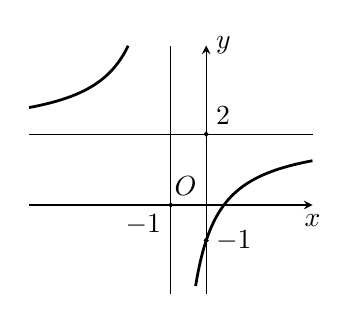
\begin{tikzpicture}[smooth,samples=300,scale=0.45,>=stealth]
			\draw[->] (-5,0)--(3,0) node[below]{$x$};
			\draw[->] (0,-2.5)--(0,4.5) node[right]{$y$};
			\draw (0,0) node[above left]{$O$};
			\draw[line width=1pt,domain=-0.3:3] plot(\x,{(2*\x-1)/(\x+1)});
			\draw[line width=1pt,domain=-5:-2.2] plot(\x,{(2*\x-1)/(\x+1)});
			\draw[fill=black] (0,2) circle(1.5pt) (0,-1) circle(1.5pt) (-1,0) circle(1.5pt);
			\draw (-5,2)--(3,2) (-1,-2.5)--(-1,4.5);
			\draw (0,-1) node[right]{$-1$};
			\draw (-1,0) node[below left]{$-1$};
			\draw (0,2) node[above right]{$2$};
		\end{tikzpicture}
	}
	\loigiai
	{
		Đồ thị hàm số có tiệm cận đứng là $x=-1$ nên loại đáp án $ y=\dfrac{2x+1}{x-1}$.\\
		Đồ thị hàm số đi qua điểm $A(0;-1)$ nên loại đáp án $y=\dfrac{1-2x}{x+1}$ và $ y=\dfrac{2x+1}{x+1}$.
	}
\end{ex} \dongcham{1}

\begin{ex}
	\immini{Đường cong trong hình vẽ bên là đồ thị của một trong bốn hàm số sau. Hỏi đó là hàm số nào?
		\choice
		{$y=\dfrac{x-1}{x-2}$}
		{$y=x+2$}
		{$y=x^4-3x^2+1$}
		{\True $y=\dfrac{2x+1}{x-1}$}
	}{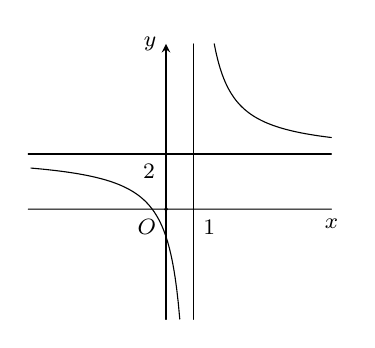
\begin{tikzpicture}[scale=0.5, line join=round, line cap=round,font=\footnotesize,>=stealth,x=0.7cm,y=0.7cm]
			\draw[fill,->] (-5,0)--(0,0) node[below left]{$O$}circle(0.05)--(6,0) node [below] {$x$};
			\draw[->] (0,-4)--(0,6) node [left] {$y$};
			\draw[black,domain=1.75:6, samples=100]plot(\x,{(2*(\x)+1)/((\x)-1)});
			\draw[black,domain=-4.9:0.5, samples=100]plot(\x,{(2*(\x)+1)/((\x)-1)});
			\draw[black,domain=-5:6, samples=100]plot(\x,{2});
			\draw[black,domain=-4:6, samples=100, variable=\t]plot(1,\t);
			\foreach \x in {1}
			\draw (\x,0.05)--(\x,-0.05) node [below right] {\x};
			\foreach \y in {2}
			\draw (0.05,\y)--(-0.05,\y) node [below left] {\y};
		\end{tikzpicture}}
	\loigiai{
		Đồ thị hàm số như hình vẽ nhận đường thẳng $x=1$ là tiệm cận đứng.\\
		Do đó, hàm số cần tìm là $y=\dfrac{2x+1}{x-1}$.
	}
\end{ex} \dongcham{1}

\begin{ex}
	\immini{Đường cong trong hình vẽ bên là đồ thị của một trong bốn hàm số sau. Hỏi đó là đồ thị của hàm số nào?
		\haicot
		{$y=\dfrac{x-2}{x+1}$}
		{$y=\dfrac{x+2}{x-2}$}
		{\True $y=\dfrac{x-2}{x-1}$}
		{$y=\dfrac{x+2}{x-1}$}
	}
	{
		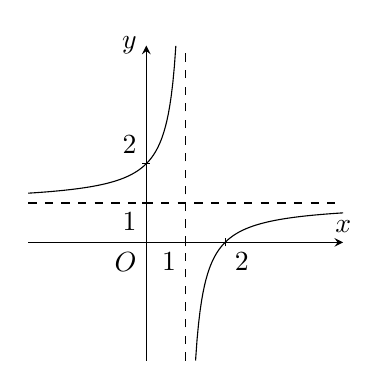
\begin{tikzpicture}[>=stealth,x=1cm,y=1cm,scale=0.5]
			\draw[->] (-3,0)--(0,0) node[below left]{$O$}--(5,0) node[above]{$x$};
			\draw[->] (0,-3) --(0,5) node[left]{$y$};
			\foreach \x in {1,2}{\draw[-] (\x,-0.1)--(\x,0.1);}
			\foreach \y in {1,2}{\draw[-] (-0.1,\y)--(0.1,\y);}
			\draw [domain=-3:0.75, samples=100] plot (\x, {(\x-2)/(\x-1)});
			\draw [domain=1.25:5, samples=100] plot (\x, {(\x-2)/(\x-1)});
			\draw [dashed](-3,1)--(5,1) (1,-3)--(1,5);
			\draw (0,1) node[below left]{$1$};
			\draw (0,2) node[above left]{$2$};
			\draw (1,0) node[below left]{$1$};
			\draw (2,0) node[below right]{$2$};
		\end{tikzpicture}
	}
	\loigiai{
		Từ đồ thị ta thấy
		\begin{itemize}
			\item Tiệm cận ngang là $y=1$, tiệm cận đứng là $x=1$ nên các hàm số $y=\dfrac{x+2}{x-2}$, $y=\dfrac{x-2}{x+1}$ không thỏa mãn.
			\item Giao điểm của đồ thị với trục tung là $(0;2)$ nên hàm số $y=\dfrac{x+2}{x-1}$ không thỏa mãn, hàm số $y=\dfrac{x-2}{x-1}$ thỏa mãn.
		\end{itemize}
	}
\end{ex} \dongcham{1}


\begin{ex}
	\immini
	{Cho hàm số $y=\dfrac{ax-b}{x+c}$ ($a,b,c\in \mathbb{R}$) có đồ thị như hình vẽ bên. Giá trị của biểu thức $2a+b-3c$ bằng
		\haicot
		{$-3$}
		{$4$}
		{\True $7$}
		{$-5$}
	}
	{\begin{tikzpicture}[scale=0.7, font=\footnotesize, line join=round, line cap=round, >=stealth]
			\def\xt{-2.5} \def\xp{4.5} \def\yt{4.5} \def\yd{-2.5}
			\draw[->] (\xt,0)--(\xp,0) node [below]{$x$};
			\draw[->] (0,\yd)--(0,\yt) node [left]{$y$};
			\node at (0,0) [below left]{$O$};
			\clip (\xt,\yd) rectangle (\xp,\yt);
			\draw[smooth,samples=200,domain=\xt:0.99] plot(\x,{(\x-2)/(\x-1)});
			\draw[smooth,samples=300,domain=1.01:\xp] plot(\x,{(\x-2)/(\x-1)});
			\draw[dashed] (1,\yd)--(1,\yt);
			\draw[dashed] (\xt,1)--(\xp,1);
			\fill (1,0)node[shift={(-120:0.3)}]{$1$} circle(1pt);
			\fill (2,0)node[shift={(-60:0.3)}]{$2$} circle(1pt);
			\fill (0,1)node[shift={(230:0.3)}]{$1$} circle(1pt);
			\fill (0,2)node[shift={(150:0.3)}]{$2$} circle(1pt);
		\end{tikzpicture}}
	\loigiai
	{Từ đồ thị hàm số ta có:\\
		Đường tiệm cận đứng là $x=1$ nên $-c=1 \Leftrightarrow c=-1$.\\
		Đường tiệm cận ngang là $y=1$ nên $a=1$.\\
		Đồ thị hàm số đi qua điểm $(0;2)$ nên $\dfrac{-b}{c}=2 \Leftrightarrow b=2$.\\
		Vậy $2a+b-3c = 2+2+3=7$.}
\end{ex} \dongcham{1}

\begin{ex}
	\immini{Cho hàm số $ y=\dfrac{ax+1}{bx-2} $ có đồ thị như hình vẽ. Tính $T=a+b$
		\haicot
		{\True $ T=2 $}
		{$ T=0 $}
		{$ T=-1 $}
		{$ T=3 $}}{
		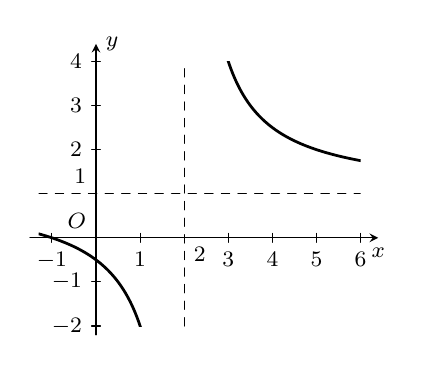
\begin{tikzpicture}[scale=0.8, font=\footnotesize, line join=round, line cap=round, >=stealth,x=0.7cm,y=0.7cm]
			\def\xmin{-1.3}\def\xmax{6}\def\ymin{-2}\def\ymax{4}
			\draw[->] (\xmin-0.2,0)--(\xmax+0.4,0) node[below] {\footnotesize $x$};
			\draw[->] (0,\ymin-0.2)--(0,\ymax+0.4) node[right] {\footnotesize $y$};
			\draw (0,1) node [above left] {\footnotesize $1$};
			\draw (2,0) node [below right] {\footnotesize $2$};
			\draw (0,0) node [above left] {\footnotesize $O$};
			\foreach \x in {-1,1,3,4,5,6}\draw (\x,0.1)--(\x,-0.1) node [below] {\footnotesize $\x$};
			\foreach \y in {-2,-1,2,3,4}\draw (0.1,\y)--(-0.1,\y) node [left] {\footnotesize $\y$};
			\clip (\xmin,\ymin) rectangle (\xmax,\ymax);
			\draw[dashed] (\xmin,1.0)--(\xmax,1.0);
			\draw[dashed] (2.0,\ymin)--(2.0,\ymax);
			\draw[line width=1pt,smooth,samples=200,domain=\xmin:1.5] plot (\x,{(1*(\x)+1)/(1*(\x)+-2)});
			\draw[line width=1pt,smooth,samples=200,domain=2.3:\xmax] plot (\x,{(1*(\x)+1)/(1*(\x)+-2)});
		\end{tikzpicture}
	}
	\loigiai{
		Từ biểu thức của hàm số, suy ra tiệm cận đứng là $ x=\dfrac{2}{b} $, tiệm cận ngang là $ y=\dfrac{a}{b} $.\\
		Dựa vào hình vẽ, suy ra tiệm cận đứng $ x=2 $, tiệm cận ngang $ y=1 $.\\
		Từ hai điều trên suy ra $ a=1 $, $ b=1 $. Vậy $ T=1+1=2 $.
	}
\end{ex} \dongcham{1}

\begin{ex}
	\immini{
		Cho hàm số $y=\dfrac{ax-b}{cx+2}$ ($a$, $b$, $c\in\mathbb{R}$; $c\neq 0$) có đồ thị như hình vẽ bên. Giá trị của biểu thức $a+b+c$ bằng
		\choice
		{$-3$}
		{$5$}
		{$-4$}
		{\True $3$}
	}{
		\begin{tikzpicture}[scale=0.7, font=\footnotesize, line join=round, line cap=round, >=stealth]
			\def\a{1} \def\b{-3} \def\c{-1} \def\d{2} % Hệ số
			\def\xt{-2} \def\xp{6} \def\yt{2} \def\yd{-4} % x_trái, x_phải, y_trên, y_dưới (giới hạn)
			\draw[->] (\xt,0)--(\xp,0) node [below]{$x$};
			\draw[->] (0,\yd)--(0,\yt) node [left]{$y$};
			\fill (0,0) circle (1.5pt) node[above left]{$O$} (1,0) circle (1.5pt) node[below]{$1$} (2,0) circle (1.5pt) node[below left]{$2$} (3,0) circle (1.5pt) node[below]{$3$} (0,-1) circle (1.5pt) node[above left]{$-1$} (0,-1.5) circle (1.5pt) node[below left]{$-\dfrac{3}{2}$};
			\clip (\xt+0.1,\yd+0.1) rectangle (\xp-0.1,\yt-0.1);
			\draw[smooth,samples=300,domain=\xt:(-\d/\c-0.1)] plot(\x,{(\a*(\x)+\b)/(\c*(\x)+\d)});
			\draw[smooth,samples=300,domain=(-\d/\c+0.1:\xp)] plot(\x,{(\a*(\x)+\b)/(\c*(\x)+\d)});
			\draw[dashed] (-\d/\c,\yd)--(-\d/\c,\yt);
			\draw[dashed] (\xt,\a/\c)--(\xp,\a/\c);
		\end{tikzpicture}
	}
	\loigiai{
		Từ hình vẽ, ta thấy đồ thị hàm số có
		\begin{itemize}
			\item Đường tiệm cận đứng $x=2$, suy ra $-\dfrac{2}{c}=2 \Leftrightarrow c=-1$.
			\item Đường tiệm cận ngang $y=-1$, suy ra $\dfrac{a}{c}=-1 \Leftrightarrow a=-c=1$.
			\item Giao điểm với trục $Oy$ tại điểm $\left(0;-\dfrac{3}{2}\right)$, suy ra $-\dfrac{b}{2}=-\dfrac{3}{2} \Leftrightarrow b=3$.
		\end{itemize}
		Vậy $a+b+c=1+3-1=3$.
	}
\end{ex} \dongcham{1}

\begin{ex}
	\immini{Hãy xác định $a$, $b$ để hàm số $y = \dfrac{2 - ax}{x + b}$ có đồ thị như hình vẽ?
		\choice
		{$a = 1$; $b = - 2$}
		{$a = b = 2$}
		{\True $a = - 1$; $b = -2$}
		{$a = b = -2$}}{

		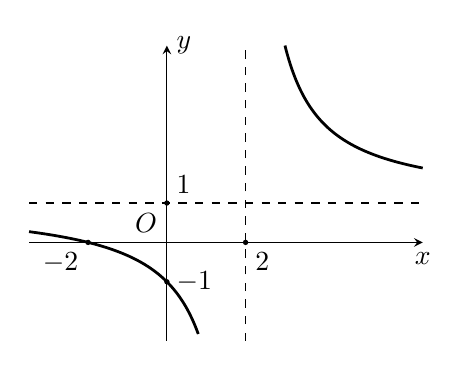
\begin{tikzpicture}[smooth,samples=300,scale=0.5,>=stealth]
			\draw[->] (-3.5,0)--(6.5,0) node[below]{$x$};
			\draw[->] (0,-2.5)--(0,5) node[right]{$y$};
			\draw (0,0) node[above left]{$O$};
			\draw[line width=1pt,domain=-3.5:0.8] plot(\x,{(\x+2)/(\x-2)});
			\draw[line width=1pt,domain=3:6.5] plot(\x,{(\x+2)/(\x-2)});
			\draw[fill=black] (0,1) circle(1.5pt) (-2,0) circle(1.5pt) (2,0) circle(1.5pt) (0,-1) circle(1.5pt);
			\draw [dashed](-3.5,1)--(6.5,1) (2,-2.5)--(2,5);
			\draw (0,-1) node[right]{$-1$};
			\draw (2,0) node[below right]{$2$};
			\draw (-2,0) node[below left]{$-2$};
			\draw (0,1) node[above right]{$1$};
		\end{tikzpicture}
	}
	\loigiai{
		Đồ thị hàm số có đường tiệm cận đứng là $x = 2$ nên $b + 2 = 0 \Leftrightarrow b = -2$.\\
		Đồ thị hàm số cắt trục hoành tại điểm $\left(-2; 0\right)$ nên $2 + 2a = 0 \Rightarrow a = -1$.
	}
\end{ex} \dongcham{1}


\begin{ex}
	\immini{Cho đồ thị hàm số $y=\dfrac{ax-b}{x-1}$ như hình vẽ. Tìm khẳng định đúng?
		\haicot
		{$a<0$, $b<0$}
		{$0<b<a$}
		{\True $b<0<a$}
		{$a<b<0$}}{
		\begin{tikzpicture}[>=stealth,scale=0.4, line join=round, line
				cap=round,font=\footnotesize]
			\draw[->] (-4,0)--(6,0) node [below]{$x$};
			\draw[->] (0,-4)--(0,6) node [right]{$y$};
			\draw[fill=black] (0,0) circle (2pt) node[below left]{$O$};
			\draw[smooth,samples=300,domain=-4:0.4] plot(\x,{(\x+2)/(\x-1)});
			\draw[smooth,samples=300,domain=1.6:6] plot(\x,{(\x+2)/(\x-1)});
			\draw[dashed] (-4,1)--(6,1) (1,-4)--(1,6);
			\draw[fill=black] (1,0) circle (2pt) node[below left]{$1$};
			\draw[fill=black] (0,1) circle (2pt) node[below left]{$1$};
			\draw[fill=black] (-2,0) circle (2pt) node[below left]{$-2$};
			\draw[fill=black] (0,-2) circle (2pt) node[below left]{$-2$};
		\end{tikzpicture}}
	\loigiai{
		Hàm số có dạng $y=\dfrac{ax-b}{x-1}$.
		\begin{itemize}
			\item Tiệm cận ngang $y=1 \Rightarrow a=1$.
			\item Đồ thị đi qua $(-2;0) \Rightarrow -2a-b=0$
		\end{itemize}
		Suy ra $b<0<a$.
	}
\end{ex} \dongcham{1}

\begin{ex}
	\immini{Cho hàm số $y=\dfrac{ax+4}{bx+c}\ (a,\ b,\ c\in \mathbb{R})$ có bảng biến thiên như sau. Trong các số $a,\ b,\ c$ có bao nhiêu số dương?
		\choice
		{$0$}
		{\True $1$}
		{$2$}
		{$3$}}{
		
\begin{tikzpicture}
			\tikzset{double style/.append style = {draw=\tkzTabDefaultWritingColor,double=\tkzTabDefaultBackgroundColor,double distance=2pt}}
			\tkzTabInit[nocadre=false,lgt=1.2,espcl=2.5,deltacl=0.6]
			{$x$ /0.6, $f'(x)$ /0.6, $f(x)$ /1.5}
			{$-\infty$,$1$,$+\infty$}
			\tkzTabLine{ ,+,d,+, }
			\tkzTabVar{-/$3$,+D-/$+\infty$/$-\infty$,+/$3$}
		\end{tikzpicture}}
	\loigiai
	{
		Dựa vào bảng biến thiên, ta có $y(0)>3\Rightarrow\dfrac{4}{c}>0\Rightarrow c>0$.\\
		Đồ thị có tiệm cận đứng $x=1$ và tiệm cận ngang $y=3$ nên $\heva{& -\dfrac{c}{b}>0\\& \dfrac{a}{b}>0}\Rightarrow\heva{&b<0\\&a<0.}$\\
		Vậy $c>0$, $a<0$, $b<0$.
	}
\end{ex} \dongcham{4}

\begin{ex}%[2D1K5-1]%
	\immini
	{
		Cho hàm số $y=\dfrac{ax+b}{cx+d}$ với $a>0$ có đồ thị như hình vẽ bên. Mệnh đề nào sau đây đúng?
		\choice
		{$b<0$, $c<0$, $d<0$}
		{$b>0$, $c<0$, $d<0$}
		{$b<0$, $c>0$, $d<0$}
		{\True $b>0$, $c>0$, $d<0$}
	}
	{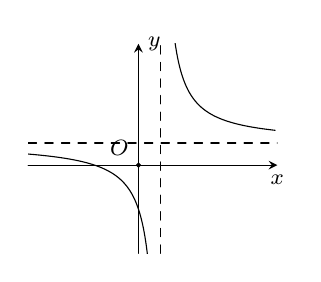
\begin{tikzpicture}[scale=0.7, font=\footnotesize, line join=round, line cap=round,>=stealth,x=0.4cm,y=0.4cm]
			\def \xmin{-5.0};
			\def \xmax{6.3};
			\def \ymin{-4.0};
			\def \ymax{5.5};
			\draw[->] (\xmin, 0.) -- (\xmax,0.) node[anchor=north] {$x$};
			\draw[->] (0.,\ymin) -- (0.,\ymax) node[anchor=west] {$y$};
			\clip(\xmin,\ymin) rectangle (\xmax,\ymax);
			\draw[smooth,samples=100,domain=\xmin-0.1:1-0.1] plot(\x,{((\x)+2)/((\x)-1)});
			\draw[smooth,samples=100,domain=1+0.1:\xmax-0.1] plot(\x,{((\x)+2)/((\x)-1)});
			\draw[dashed] (\xmin,1)--(\xmax,1) (1,\ymin)--(1,\ymax);
			\draw[fill=black] (0,0) circle (1pt) node[above left] {$O$};
		\end{tikzpicture}
	}
	\loigiai{
		Đồ thị hàm số có đường tiệm cận ngang $y=\dfrac{a}{c}$ nằm trên trục $Ox$ nên $\dfrac{a}{c}>0\overset{a>0}{\Rightarrow} c>0$.\\
		Đồ thị hàm số có đường tiệm cận đứng $x=-\dfrac{d}{c}$ nằm bên phải trục $Oy$ nên $-\dfrac{d}{c}>0\overset{c>0}{\Rightarrow}d<0$.\\
		Vậy mệnh đề đúng là \lq\lq $b>0$, $c>0$, $d<0$\rq\rq.
	}
\end{ex} \dongcham{4}

\begin{ex}
	\immini{Hình vẽ bên là đồ thị của hàm số $y=\dfrac{ax+b}{cx+d}$. Mệnh đề nào sau đây là đúng?
		\choice
		{$ab>0,bd<0$}
		{$ab<0,ad>0$}
		{\True $ab<0,ad<0$}
		{$bd>0,ad>0$}
	}{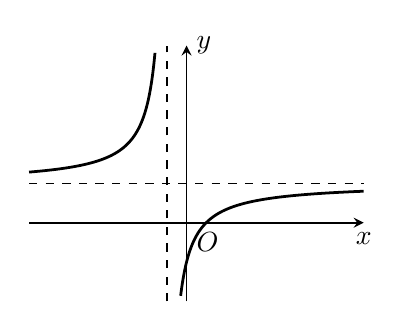
\begin{tikzpicture}[smooth,samples=300,line width=0.6pt,>=stealth, scale=0.5]
			\draw[->] (-4,0)--(4.5,0) node[below]{$x$};
			\draw[->] (0,-2)--(0,4.5) node[right]{$y$};
			\draw (0,0) node[below right]{$O$};
			\draw[dashed] (-0.5,-2)--(-0.5,4.5) (-4,1)--(4.5,1);
			\draw[line width=1pt,domain=-4:-0.8] plot(\x,{(2*(\x)-1)/(2*(\x)+1)});
			\draw[line width=1pt,domain=-0.15:4.5] plot(\x,{(2*(\x)-1)/(2*(\x)+1)});
		\end{tikzpicture}
	}
	\loigiai{
		Ta có
		\begin{itemize}
			\item [$\bullet$] Đường tiệm cận đứng $x=-\dfrac{d}{c}$. Theo hình vẽ thì $-\dfrac{d}{c}<0 \Rightarrow cd >0$ \quad (1).
			\item [$\bullet$] Đường tiệm cận ngang $y=\dfrac{a}{c}$. Theo hình vẽ thì $\dfrac{a}{c}<0 \Rightarrow ac <0$ \quad (2).
			\item [$\bullet$] Giao điểm với trục tung tại điểm có tung độ $y=\dfrac{b}{d}$. Theo hình vẽ thì $\dfrac{b}{d}>0 \Rightarrow bd >0$ \quad (3).
			\item [$\bullet$] Giao điểm với trục hoành tại điểm có hoành độ $x=-\dfrac{b}{a}$. Theo hình vẽ thì $-\dfrac{b}{a}>0 \Rightarrow ab <0$ \quad (4).
		\end{itemize}
		Lấy (3) nhân với (4), ta được $ad \cdot b^2 <0$. Suy ra $ad<0$.\\
		Mặt khác theo (4) thì $ab<0$.
	}
\end{ex} \dongcham{4}


\begin{ex}
	\immini{Hình vẽ dưới đây là đồ thị hàm số $y=\dfrac{ax+b}{cx+d}$ $ac\ne0$, $ad-cb\ne0$. Mệnh đề nào sau đây đúng?
		\choice
		{\True $ad>0$ và $ab<0$}
		{$bd<0$ và $ab>0$}
		{$ad<0$ và $ab<0$}
		{$ad>0$ và $bd>0$}
	}
	{\begin{tikzpicture}[>=stealth,font=\footnotesize,scale=0.6]
			\draw[->](-4,0)--(3,0)node[below]{$x$};
			\draw[->](0,-3.5)--(0,3)node[right]{$y$};
			\draw[smooth,samples=100,domain=-4:-1.4]plot(\x,{(\x-1)/(2*\x+2)});
			\draw[smooth,samples=100,domain=-0.75:3]plot(\x,{(\x-1)/(2*\x+2)});
			\draw(-4,0.5)--(3,0.5) (-1,-3.5)--(-1,3);
			\fill (0,0)node[below left]{$O$}circle (1.2pt);
		\end{tikzpicture}}
	\loigiai{
		\begin{itemize}
			\item Đồ thị hàm số cắt trục $Oy$ tại điểm có tung độ âm $\Rightarrow\dfrac{b}{d}< 0\Rightarrow bd<0$.
			\item Đồ thị hàm số cắt trục $Ox$ tại điểm có hoành độ dương $\Rightarrow-\dfrac{b}{a}> 0\Rightarrow ab<0$.
			\item Đồ thị hàm số có tiệm cận ngang $y=\dfrac{a}{c}>0\Rightarrow ac>0.\quad(1)$
			\item Đồ thị hàm số có tiệm cận đứng $x=-\dfrac{d}{c}<0\Rightarrow cd>0.\quad(2)$
		\end{itemize}
		Từ $(1)$ và $(2)\Rightarrow ad>0$.}
\end{ex} \dongcham{4}
\Closesolutionfile{ans}

\ind{PHẦN II.} \inden{Câu trắc nghiệm đúng sai. Trong mỗi ý a), b), c), d) ở mỗi câu, học sinh chọn đúng hoặc sai.}\\
\Opensolutionfile{ans}[ans/2D1-B4-d2-2]

\begin{ex}
	\immini{Cho hàm số $y = \dfrac{x + a}{b x +c}$, $\left( a, b, c \in \mathbb{Z}\right) $.
		\choiceTF
		{\True Đồ thị hàm số có tiệm cận đứng $x=1$}
		{Đồ thị hàm số có tiệm cận ngang $y=0$}
		{Hàm số đồng biến trên $\mathbb{R}$}
		{\True $a - 3b - 2c=-3$}
	}{
		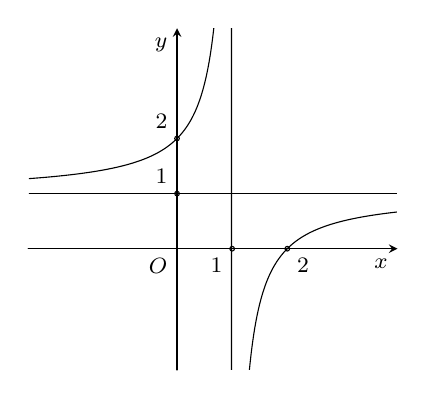
\begin{tikzpicture}[font=\footnotesize,line join=round, line cap=round,>=stealth,scale=0.7]
			\tikzset{label style/.style={font=\footnotesize}}
			\def \xmin{-2.7}
			\def \xmax{4}
			\def \ymin{-2.2}
			\def \ymax{4}
			\draw[->] (\xmin,0)--(\xmax,0) node[below left] {$x$};
			\draw[->] (0,\ymin)--(0,\ymax) node[below left] {$y$};
			\draw (0,0) node [below left] {$O$};
			\draw (1,0) node [below left] {$1$} circle (1.2pt);
			\draw (2,0) node [below right] {$2$} circle (1.2pt);
			\draw (0,1) node [above left] {$1$} circle (1.2pt);
			\draw (0,2) node [above left] {$2$} circle (1.2pt);
			\begin{scope}
				\clip (\xmin+0.01,\ymin+0.01) rectangle (\xmax-0.01,\ymax-0.01);
				\draw[samples=350,domain=\xmin+0.01:\xmax-0.01,smooth,variable=\x] plot (\x,{(\x-2)/(\x-1)});
				\draw[samples=200,domain=\xmin+0.01:\xmax-0.01,smooth,variable=\x] plot (\x,{1});
			\end{scope}
		\end{tikzpicture}
	}
	\loigiai{
		Căn cứ vào đồ thị, ta có
		\begin{enumerate}[a)]
			\item Đồ thị hàm số có tiệm cận đứng $x=1$.
			\item Đồ thị hàm số có tiệm cận ngang $y=1$
			\item Hàm số đồng biến trên các khoảng $(-\infty,1)$ và $(1;+\infty)$
			\item Đồ thị hàm số có tiệm cận ngang $y = 1$ nên $\dfrac{1}{b} = 1 \Rightarrow b = 1$.\\
			      Đồ thị hàm số có tiệm cận đứng $x = 1$ nên $-\dfrac{c}{b} = 1$ mà $b = 1$ $\Rightarrow c = -1$.\\
			      Đồ thị hàm số cắt trục tung tại điểm $(0; 2)$ nên $\dfrac{a}{c} = 2$ mà $c = -1$ nên $a = -2$.\\
			      Vậy $T = a - 3b - 2c = -2 - 3 \cdot 1 -2 \cdot (-1) =-3 $.
		\end{enumerate}

	}
\end{ex} \dongcham{4}

\begin{ex}%[2D1K5-1]%
	Cho hàm số $ f(x)=\dfrac{a x-1}{b x+c}\ (a, b, c\in\mathbb{R})$ có bảng biến thiên như sau.
	\begin{center}
		
\begin{tikzpicture}
			\tikzset{double style/.append style = {draw=\tkzTabDefaultWritingColor,double=\tkzTabDefaultBackgroundColor,double distance=2pt}}
			\tkzTabInit[espcl=2.5,lgt=1.2,nocadre=false]
			{$x $ /0.7, $ f'(x)$ /0.7, $ f(x)$ /2.1}
			{$-\infty $, $ 3 $, $+\infty$}
			\tkzTabLine{,-,d,-,}
			\tkzTabVar{+/ $\dfrac{1}{2}$,-D+/ $-\infty $ / $+\infty $,-/ $\dfrac{1}{2}$}
		\end{tikzpicture}
	\end{center}
		\choiceTF
		{\True Hàm số nghịch biến trên khoảng $\left( -\infty,\dfrac{1}{2}\right)$}
		{Đồ thị hàm số có tiệm cận đứng $x=\dfrac{1}{2}$}
		{\True Đồ thị giao với trục hoành tại điểm có hoành độ nhỏ hơn $3$}
		{\True $\hoac{&b>\dfrac{2}{3}\\ &b<0}$}
	\loigiai{
		\begin{enumerate}[a)]
			\item Hàm số đồng biến trên các khoảng $(-\infty,3)$ nên nghịch biến trên khoảng $\left( -\infty,\dfrac{1}{2}\right)$.
			\item Đồ thị hàm số có tiệm cận đứng $x=3$.
			\item Đồ thị giao với trục hoành tại điểm thuộc nhánh trái của đồ thị, suy ra hoành độ giao điểm này nhỏ hơn $3$.
			\item Từ bảng biến thiên suy ra
			      \[
				      \heva{&\dfrac{a}{b}=\dfrac{1}{2}\\&-\dfrac{c}{b}=3.}\quad\quad (1)
			      \]
			      Ta có $ y'=\dfrac{ac+b}{(bx+c)^2}<0 $, $\forall x\ne-\dfrac{c}{b}\Leftrightarrow ac+b<0 $.\quad\quad (2)\\
			      Từ (1) và (2) suy ra $\dfrac{b}{2}\cdot (-3b)+b<0\Leftrightarrow\hoac{&b>\dfrac{2}{3}\\ &b<0.}$
		\end{enumerate}
	}
\end{ex} \dongcham{4}

\begin{ex}
	\immini{Cho hàm số $f(x)=\dfrac{ax+b}{cx+d}$ với $a$, $b$, $c$, $d \in \mathbb{R}$ có đồ thị hàm số $y=f'(x)$ nhận $x=-1$ làm tiệm cận đứng như hình vẽ bên. Biết rằng giá trị lớn nhất của hàm số $y=f(x)$ trên đoạn $[-3;-2]$ bằng $8$.
		\choiceTF
		{\True $f'(0)=3$}
		{Hàm số $f(x)$ nghịch biến trên khoảng $(-1;+\infty)$}
		{Giá trị của $f(-3)$ bằng $8$}
		{\True  Giá trị của $f(2)$ bằng $4$}
	}
	{\begin{tikzpicture}[>=stealth,scale=0.6, line join=round, line cap=round]
			\def\a{3} \def\b{0} \def\c{1} \def\d{1} % Hệ số
			\def\xt{-4.5} \def\xp{4.5} \def\yt{5.5} \def\yd{-1}
			\draw[->] (\xt,0)--(\xp,0) node [below]{$x$};
			\draw[->] (0,\yd)--(0,\yt) node [left]{$y$};
			\node at (0,0) [below left]{$O$};
			\clip (\xt-0.1,\yd+0.1) rectangle (\xp-0.1,\yt-0.1);
			\draw[smooth,samples=300,domain=\xt:(-\d/\c-0.1)] plot(\x,{(\a)/(\c*(\x)+\d)^2});
			\draw[smooth,samples=300,domain=(-\d/\c+0.1:\xp)] plot(\x,{(\a)/(\c*(\x)+\d)^2});
			\draw (-\d/\c,\yd)--(-\d/\c,\yt);
			\draw (-1,0) node [below left] {$-1$} circle (1.2pt)
			(0,3) node [right] {$3$} circle (1.2pt);
		\end{tikzpicture}}
	\loigiai{
		\begin{enumerate}[a)]
			\item Theo hình vẽ, đồ thị $f'(x)$ qua điểm $(0;3)$ nên $f'(0)=3$.
			\item Do $f'(x)>0$, $\forall x \ne -1$ nên hàm số $f(x)$ đồng biến trên các khoảng $(-\infty;-1)$ và $(-1;+\infty)$.
			\item Vì $f'(x)>0$, $\forall x \ne -1 \Rightarrow \max \limits_{[-3;-2]} f(x)=f(-2)=8$. Suy ra $f(-3) \ne 8$.
			\item Ta có $f'(x)=\dfrac{ad-bc}{(cx+d)^2}$.\\
			      Đồ thị hàm số đi qua điểm $(0;3)$ nên $f'(0)=3 \Leftrightarrow \dfrac{ad-bc}{d^2}=3$.\\
			      Mặt khác, đồ thị hàm số $y=f'(x)$ có tiệm cận đứng $x=-1$ nên $-c+d=0$.\\
			      Vì $f'(x)>0$, $\forall x \ne -1 \Rightarrow \max \limits_{[-3;-2]} f(x)=f(-2)=8 \Leftrightarrow \dfrac{-2a+b}{-2c+d}=8$.\\
			      Vậy ta có hệ phương trình $\heva{&ad-bc=3d^2\\&-c+d=0\\&b-2a=8(d-2c)}\Leftrightarrow\heva{&c=d\\&a-b=3d\\&b-2a=-8d}\Leftrightarrow\heva{&a=5d\\&b=2d\\&c=d.}$\\
			      Từ đó suy ra $f(x)=\dfrac{5\mathrm{\,d}x+2d}{\mathrm{\,d}x+d}=\dfrac{5x+2}{x+1} \Rightarrow f(2)=4$.
		\end{enumerate}
	}
\end{ex} \dongcham{5}
\Closesolutionfile{ans}